\documentclass[10pt]{article}
\usepackage[utf8]{inputenc}
\usepackage[T1]{fontenc}
\usepackage{graphicx}
\usepackage[export]{adjustbox}
\graphicspath{ {./images/} }
\usepackage{amsmath}
\usepackage{amsfonts}
\usepackage{amssymb}
\usepackage{mhchem}
\usepackage{stmaryrd}
\usepackage{hyperref}
\hypersetup{colorlinks=true, linkcolor=blue, filecolor=magenta, urlcolor=cyan,}
\urlstyle{same}

\title{Chapter 1 }

\author{}
\date{}


\begin{document}
\maketitle
\section{Distribution System Regulations}
Drinking water regulations have undergone major and dramatic changes during the past two decades, and trends indicate that they will continue to become more stringent and complicated. It is important that all water system operators understand the basic reasons for having regulations, how they are administered, and why compliance with them is essential. The reader should recognize that regulatory requirements are constantly changing. It is the operator's responsibility to keep current on all regulatory requirements.

\section{FEDERAL REGULATIONS}
Although the regulations required by the Safe Drinking Water Act (SDWA) are of prime interest in the operation and administration of water distribution systems, operators must also adhere to regulations required by several other federal environmental and safety acts.

\section{Safe Drinking Water Act Requirements}
Requirements under the SDWA are quite extensive, and complete details can be found in publications (and websites) listed in the bibliography at the end of this chapter. The SDWA includes a number of (current and proposed) rules including the following:

\begin{itemize}
  \item Surface Water Treatment Rule (SWTR)

  \item Total Coliform Rule (TCR)

  \item Interim Enhanced Surface Water Treatment Rule (IESWTR)

  \item Long-Term 1 Enhanced Surface Water Treatment Rule (LT1ESWTR)

  \item Long-Term 2 Enhanced Surface Water Treatment Rule (LT2ESWTR)

  \item Ground Water Rule (GWR)

  \item Total Trihalomethane (TTHM) Rule

  \item Stage 1 Disinfectants/Disinfection By-products Rule (Stage 1 DBPR)

  \item Stage 2 Disinfectants/Disinfection By-products Rule (Stage 2 DBPR)

  \item Lead and Copper Rule (LCR)

  \item Public Notification (PN) Rule - Filter Backwash Recycle Rule (FBRR)

  \item Unregulated Contaminant Monitoring Rule (UCMR)

\end{itemize}
The following discussion will primarily center on requirements that affect the operation of water distribution systems.

Prior to 1975, review of public water supplies was done by each state, usually by the state health department. The SDWA was passed by Congress in 1975 for a combination of reasons. One of the primary purposes was to create uniform national standards for drinking water quality to ensure that every public water supply in the country would meet minimum health standards. Another was that scientists and public health officials had recently discovered many previously unrecognized disease organisms and chemicals that could contaminate drinking water and might pose a health threat to the public. It was considered beyond the capability of the individual states to deal with these problems.

The SDWA delegates responsibility for administering the provisions of the act to the US Environmental Protection Agency (USEPA). The agency is headquartered in Washington, D.C., and has 10 regional offices in major cities of the United States. Some principal duties of the agency are to

\begin{itemize}
  \item Set maximum allowable concentrations for contaminants that might present a health threat in drinking water-these are called maximum contaminants levels (MCLs);

  \item Delegate primary enforcement responsibility for local administration of the requirements to state agencies;

  \item Provide grant funds to the states to assist them in operating the greatly expanded program mandated by the federal requirements;

  \item Monitor state activities to ensure that all water systems are being required to meet the federal requirements; and

  \item Provide continued research on drinking water contaminants and improvement of treatment methods.

\end{itemize}
\section{State Primacy}
The intent of the SDWA is for each state to accept primary enforcement responsibility (primacy) for the operation of the state's drinking water program. Under the provisions of the delegation, the state must establish requirements for public water systems that are at least as stringent as those set by USEPA. The primacy agency in each state was designated by the state governor. In some states the primacy agency is the state health department, and in others it is the state environmental protection agency, department of natural resources, or pollution control agency. USEPA has primacy in any state (e.g., Wyoming) that has not accepted this role.

\section{Classes of Public Water Systems}
The basic definition of a public water system in the SDWA is, in essence, a system that supplies piped water for human consumption and has at least

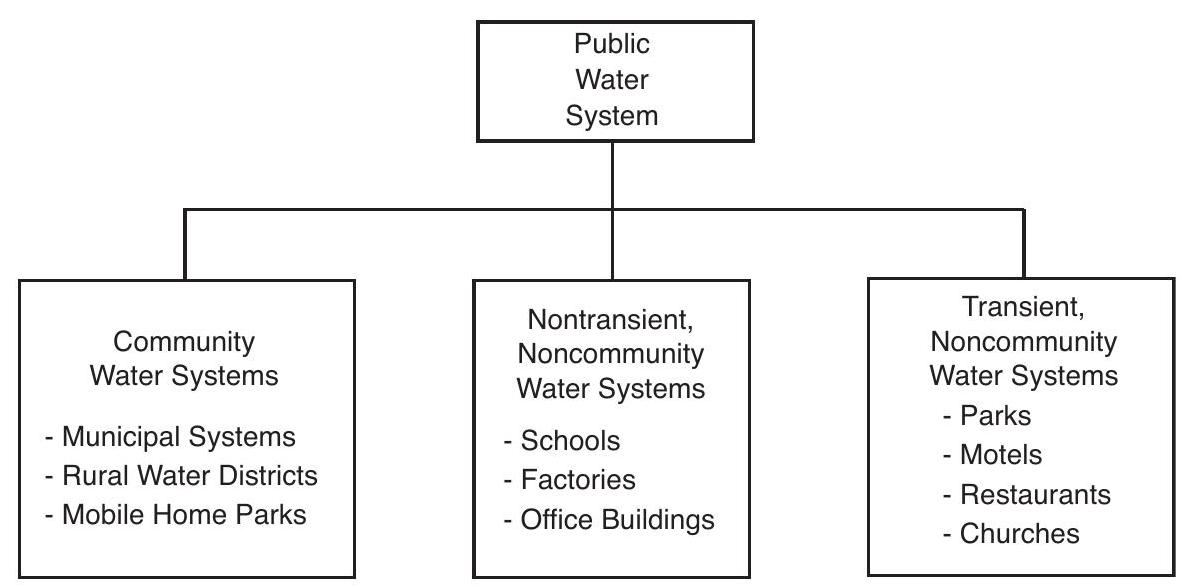
\includegraphics[max width=\textwidth]{2022_09_17_867b38c7c364bb842283g-03}

Source: Drinking Water Handbook for Public Officials (1993).

Figure 1-1 Classification of public water systems

15 service connections or serves 25 or more persons for 60 or more days of the year. Examples of water systems that would not fall under the federal definition are private homes, groups of fewer than 15 homes using the same well, and summer camps that operate for fewer than 60 days per year. These systems are, however, generally under some degree of supervision by a local, area, or state health department.

USEPA has further divided public water systems into three classifications (Figure 1-1):

\begin{enumerate}
  \item Community public water systems serve 15 or more homes. Besides municipal water utilities, this classification also covers mobile home parks and small homeowner associations that have their own water supply and serve more than 15 homes.

  \item Nontransient, noncommunity public water systems are establishments that have their own private water systems, serving an average of at least 25 persons who do not live at the location, but the same people use the water for more than 6 months per year. Examples are schools and factories.

  \item Transient, noncommunity public water systems are establishments such as parks and motels that have their own water systems and serve an average of at least 25 persons per day, but these persons use the water only occasionally and for short periods of time.

\end{enumerate}
The monitoring requirements for community and nontransient, noncommunity systems include all contaminants that are considered a public health threat. Transient, noncommunity systems are only required to monitor for nitrate, nitrite, and microbiological contamination.

\section{Regulation of Contaminants}
The National Primary Drinking Water Regulations (NPDWRs) specify MCLs or a treatment technique requirement for contaminants that may be found in drinking water and could have an adverse health effect on humans.

Specific concentration limits for the chemicals are listed, and all community and nontransient, noncommunity systems must test for their presence. If a water system is found to have concentrations of chemicals present that are above the MCL, the system must either change its water source or treat the water to reduce the chemical concentration. Primary regulations are mandatory and must be complied with by all water systems to which they apply.

The National Secondary Drinking Water Regulations apply to drinking water contaminants that may adversely affect the aesthetic qualities of water, such as taste, odor, or color. These qualities have no known adverse health effects, but they seriously affect public acceptance of the water. Secondary regulations are not mandatory but are strongly urged by USEPA. Some state regulatory agencies have made some of the secondary limits mandatory in their states.

\section{Public Notification}
The SDWA mandates that the public be kept informed of noncompliance with federal requirements by requiring that noncomplying systems provide public notification. If public water systems violate any of the operating, monitoring, or reporting requirements, or if the water quality exceeds an MCL, the system must inform the public of the problems. Even though the problem may have already been corrected, an explanation must be provided in the news media describing the public health significance of the violation.

The language and methods of providing public notification are mandated by USEPA to ensure that the public is fully informed. If a system is required to provide public notification, the state primacy agency will provide full instructions.

Water distribution operators should understand that, although public notification is intended to keep the public informed, if it is caused by a simple mistake such as forgetting to send in the monthly samples, it can cause some embarrassment for the system's staff. To avoid this situation, careful attention must be given to state requirements. If there is any problem in meeting any of the requirements, it should be discussed with the state agency representative.

If an operator is required to provide public notification, it should be made as positive as possible. Although the basic wording is mandatory, other wording can be added to keep it from sounding completely negative to the public. Such wording can be discussed with the primacy agency representative.

\section{Monitoring and Reporting}
To ensure that the drinking water supplied by all public water systems meets federal and state requirements, system operators are required to regularly collect samples and have the water tested. The regulations specify minimum sampling frequencies, sampling locations, testing procedures, methods of keeping records, and frequency of reporting to the state. The regulations also mandate special reporting procedures to be followed if a contaminant exceeds an MCL.

All systems must provide periodic monitoring for microbiological contaminants and some chemical contaminants. The frequency of sampling and the chemicals that must be tested for depend on the size of the water system, the source of water, and the history of analyses.

State policies vary on providing laboratory services. Some states have the laboratory facilities available to perform all required analyses or, in some cases, a certain number of the required analyses for a system. Most states charge for all or some of the laboratory services. Sample analyses that are required and cannot be performed by a state laboratory must be taken or sent to a state-certified private laboratory.

If the analysis of a sample exceeds an MCL, resampling is required, and the state should be contacted immediately for special instructions. There is always a possibility that such a sample was caused by a sampling or laboratory error, but it must be handled as though it was actually caused by contamination of the water supply.

The results of all water analyses must be periodically sent to the state. Failure to have the required analyses performed or to report the results to the state will usually result in the system having to provide public notification. States typically have special forms for submitting the data and specify a number of days following the end of the monitoring period by which the form must be submitted. The minimum information that must be provided in the form is listed in Table 1-1. State regulators may also require other information for their own records and documentation.

Table 1-1 Laboratory report summary requirements

\begin{tabular}{ll}
\hline
Type of Information & Summary Requirement \\
\hline
Sampling information & Date, place, and time of sampling \\
 & Name of sample collector \\
 & Identification of sample \\
 & - Routine or check sample \\
 & - Raw or treated water \\
Analysis information & Date of analysis \\
 & Laboratory conducting analysis \\
 & Name of person responsible for analysis \\
 & Analytical method used \\
 & Analysis results \\
\hline
\end{tabular}

Table 1-2 Record-keeping requirements

\begin{tabular}{ll}
\hline
Type of Records & Time Period \\
\hline
Bacteriological and turbidity analyses & 5 years \\
Chemical analyses & 10 years \\
Actions taken to correct violations & 3 years \\
Sanitary survey reports & 10 years \\
Exemptions & 5 years following expiration \\
\hline
\end{tabular}

There are also specific requirements for the length of time a water system must retain records. Table 1-2 lists the record-keeping requirements mandated by USEPA.

\section{Water Quality Monitoring}
Although most water quality monitoring is related to ensuring proper quality of the source water or treatment processes, many of the samples are collected from the distribution system. Thus, sample collection often becomes a duty of distribution system personnel. The reason for collecting samples from the distribution system is that there are some opportunities for water quality to change after it enters the distribution system, and under the requirements of the SDWA, it is the duty of the water purveyor to deliver water of proper quality to the consumer's tap.

\section{Methods of Collecting Samples}
Two basic methods of collecting samples are grab sampling and composite sampling. A grab sample is a single volume of water collected at one time from a single place. To sample water in the distribution system, a faucet is used to fill a bottle. This sample represents the quality of the water only at the time the sample was collected. If the quality of the water is relatively uniform, the sample will be quite representative. If the quality varies, the sample may not be representative.

A composite sample consists of a series of grab samples collected from the same point at different times and mixed together. The composite is then analyzed to obtain the average value. If the composite sample is made up of equal-volume samples collected at regular intervals, it is called a time composite sample. Another method is to collect samples at regular time intervals, but the size of each grab sample is proportional to the flow at the time of sampling. This is called a flow-proportional composite sample.

Although composite sampling appears to be a good idea because it provides an average of water quality, it cannot be used for most analyses of drinking water quality because a majority of parameters are not stable over a period of time.

\section{Sample Storage and Shipment}
Care must always be taken to use the exact sample containers specified or provided by the laboratory that will be doing the analyses. Most sample containers are now plastic to avoid the possibility of glass breaking during shipment. Some samples for organic chemical analysis must be collected in special glass containers because some of the chemical might permeate the walls of a plastic container.

Sample holding time before analysis is quite critical for some parameters. If a laboratory receives a sample that has passed the specified holding time, it is supposed to declare the sample invalid and request resampling. Some samples can be refrigerated or treated once they arrive at the laboratory to extend the holding time, allowing the laboratory a few more days before the analyses must be completed.

Many laboratories do not work on weekends, so this should be taken into consideration when sending samples. Bacteriological analyses must, for example, be performed immediately by the laboratory. The best time to collect and send these samples is on a Monday or Tuesday so they will reach the laboratory by mid-week. Samples should be sent to the laboratory by the fastest means available, such as first-class mail or special carrier.

\section{Sample Point Selection}
Samples are collected from various points in the distribution system to determine the quality of water delivered to consumers. In some cases, distribution system samples may be significantly different from samples collected as the water enters the system. For example, corrosion in pipelines, bacterial growth, or algae growth in the pipes can cause increases in color, odor, turbidity, and chemical content (e.g., lead and copper). More seriously, a cross-connection between the distribution system and a source of contamination can result in chemical or biological contamination of the water.

Most samples collected from the distribution system will be used to test for coliform bacteria and chlorine residual. The two primary considerations in determining the number and location of sampling points are that they should be

\begin{enumerate}
  \item Representative of each different source of water entering the system (i.e., if there are several wells that pump directly into the system, samples should be obtained that are representative of the water from each one); and

  \item Representative of the various conditions within the system (such as dead ends, loops, storage facilities, and each pressure zone).

\end{enumerate}
The required number of samples that must be collected and the frequency of sampling depend on the number of customers served, the water source, and other factors. Specific sampling instructions must be obtained from the state primacy agency.

\section{Sample Faucets}
After representative sample points have been located on the distribution system, specific locations having suitable faucets for sampling must be identified. If suitably located, public buildings and the homes of utility employees are convenient places to collect samples. Otherwise, arrangements must be made to collect samples from businesses or private homes.

The following types of sampling faucets should not be used:

\begin{itemize}
  \item Any faucet located close to the bottom of a sink, because containers may touch the faucet

  \item Any leaking faucet with water running out from around the handle and down the outside

  \item Any faucet with threads, such as a sill cock, because water generally does not flow smoothly from them and may drip contamination from the threads

  \item Any faucet connected to a home water-treatment unit, such as a water softener or carbon filter

  \item Drinking fountain

\end{itemize}
It is also best to try to find a faucet without an aerator. If faucets with aerators must be used, follow the state recommendations on whether or not the aerator should be removed for sampling.

Each sample point must be described in detail on the sample report form-not just the house address, but which faucet in which room. If resampling is necessary, the same faucet used for the first sample must be used.

When it is necessary to establish a sampling point at a location on the water system where no public building or home gives access for regular sampling, a permanent sampling station can be installed (Figure 1-2).\\

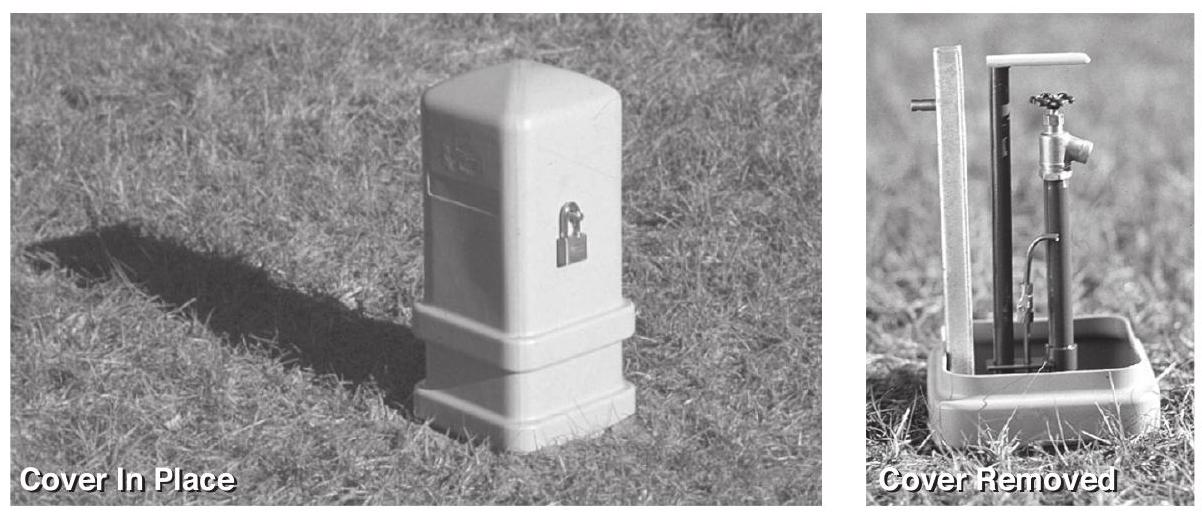
\includegraphics[max width=\textwidth]{2022_09_17_867b38c7c364bb842283g-08}

Courtesy of Gil Industries, Inc.

Figure 1-2 Example of a permanent sampling station

\section{Sample Collection}
For collection of bacteriological and most other samples, the procedure is to open the faucet so that it will produce a steady, moderate flow. Opening the faucet to full flow for flushing is not usually desirable because the flow may not be smooth and water will splash up onto the outside of the spout. If a steady flow cannot be obtained, the faucet should not be used.

The water should be allowed to run long enough to flush any stagnant water from the house plumbing, which usually takes 2 to 5 minutes. The line is usually clear when the water temperature drops and stabilizes. The sample is then collected without changing the flow setting. The sample container lid should be held (not set down on the counter) with the threads down during sample collection and replaced immediately. The sample container should then be labeled.

The exception to the above-mentioned procedure is sampling for lead and copper analysis. These are to be first-draw samples and require special procedures.

Bottles to be used for collection of bacteriological samples should not be rinsed before they are filled. These bottles are usually prepared with a small quantity of thiosulfate at the bottom to immediately stop the action of the residual chlorine in the water.

\section{Special-Purpose Samples}
It is occasionally necessary to collect special samples, particularly in response to customer complaints, such as taste and odor issues. To check on this type of complaint, one sample should be collected immediately as the tap is opened to be representative of water that has been in the plumbing system, then a second sample should be collected after the line has been flushed. It is sometimes helpful to collect both hot- and cold-water samples in this manner. These samples can be used to identify whether the problem is in the customer's plumbing system or coming from the water distribution system. Many customer complaints of taste, odor, or color are found to be from their own water heaters, water softeners, or home water-treatment devices.

\section{Laboratory Certification}
It is imperative that the monitoring of all water systems be consistent; therefore, all laboratory analyses must be performed by experienced technicians under carefully controlled conditions. For this reason, compliance sample analyses are acceptable to the state only if they have been performed by a certified laboratory. The only exceptions are measurements for turbidity, chlorine residual, temperature, and $\mathrm{pH}$, which may be performed by a person acceptable to the state, using approved equipment and methods.

Most states operate certified laboratories that can accept some or all of the samples from water systems. The states also certify private laboratories that may be used for performing water analyses. Most large water utilities have their own certified laboratories because of the great number of samples that must be processed.

\section{Consumer Confidence Reports}
One of the very significant provisions of the 1996 SDWA Amendments is the consumer confidence report (CCR) requirement. The purpose of the CCR is to provide all water customers with basic facts regarding their drinking water so that individuals can make decisions about water consumption based on their personal health. This directive has been likened to the requirement that packaged food companies disclose what is in their food products.

The reports must be prepared yearly by every community water system. Water systems serving more than 10,000 people must mail the report to customers. Smaller systems must notify customers as directed by the state primacy agency.

A water system that only distributes purchased water (satellite system) must prepare the report for their consumers. Information on the source water and chemical analyses must be provided to the satellite system by the system selling the water (parent system).

Some states are preparing much of the information for their water systems, but the system operator must still add local information. Water system operators should keep in mind that CCRs provide an opportunity to educate consumers about the sources and quality of their drinking water. Educated consumers are more likely to help protect drinking water sources and be more understanding of the need to upgrade the water system to make their drinking water safe.

\section{USEPA Regulation Information}
Current information on USEPA regulations can be obtained by contacting the Safe Drinking Water Hotline at 800-426-4791. Also see the Office of Ground Water and Drinking Water Web page at \href{http://water.epa.gov/drink}{http://water.epa.gov/drink}.

\section{STATE REGULATIONS}
Under the provisions of primacy delegation, each state must have requirements applying to public water systems that are at least as stringent as those set by USEPA. States occasionally establish requirements that are more stringent. Federal requirements are only for factors that USEPA considers directly related to public health. So, in addition to the federal requirements, each state also establishes other requirements to ensure proper water system operation.

\section{Operator Certification}
One requirement of the 1996 SDWA Amendments is that USEPA must establish minimum standards for state operator certification programs. Most states have had some form of certification for water system operators, but, unfortunately, each state has its own idea of how operators should be classified, so there has been little national consistency.

Among the more important requirements are that each water system must at all times be under the direct supervision of a certified operator, operators must have a high school or equivalent education and pass an examination to receive certification, and the state must establish training requirements for certification renewal. Most states have a separate certification class for distribution system operators.

\section{Cross-Connection Control}
The states also generally promote cross-connection control programs for all water systems. Many states have their own cross-connection control manuals and assist water systems in setting up local programs. Cross-connection control is covered in detail in chapter $13 .$

\section{Construction Approval}
The SDWA requires states to review plans for water system construction and improvements. In general, plans and specifications for the proposed work must be prepared by a professional engineer and submitted for approval before work begins. State engineers review the plans for suitability of materials, conformance with state regulations, and other factors.

Some states allow small distribution system additions without approval or allow approval after construction. State regulations should be reviewed to ensure compliance with requirements.

\section{Technical Assistance}
One of the staff functions of the state drinking water program is to provide technical assistance to water system operators. Field staff with training and experience are usually available to provide advice and assistance. If possible, they will provide advice over the phone, but if the problem is of sufficient magnitude, they will arrange personal visits. Staff may also, on some occasions, suggest other sources of information or assistance.

\section{Enforcement}
Because of the direct relationship between drinking water quality and public health, it is rare for anyone to purposely disregard state and federal regulations. Most violations of regulations are caused by not understanding requirements or forgetting something that must be done.

The SDWA requires states to use enforcement actions when federal requirements are violated. Then if the state does not take appropriate action, USEPA is prepared to step in and do it. Minor infractions are handled by public notification, but intentional disregard for requirements can result in substantial monetary fines.

\section{REQUIREMENTS OF SPECIAL INTEREST TO DISTRIBUTION SYSTEM OPERATORS}
Distribution system regulations address three main areas of concern: microbiological safety, disinfection by-products (DBPs), and lead. The microbiological safety of the water reaching customers' taps is of primary concern, and this was the initial focus of the distribution system regulatory requirements.

DBPs, such as total trihalomethanes (TTHM), are created by chemical reactions between disinfectants (like chlorine) and other substances in the water. High levels in water may increase the risk of cancer for some individuals over a lifetime. Therefore, MCLs and monitoring requirements are included in the appropriate rules. These requirements are changing as more is learned about the levels of concern.

Lead is hazardous if consumed in high amounts, particularly for children. Water with certain characteristics may dissolve lead from solder or plumbing fixtures (or lead service lines) and may pose a risk to consumers. Therefore, special tap sampling requirements are mandated to determine the need to stabilize the water or perhaps replace lead water services. The applicable regulatory rules are discussed in more detail in the following sections.

\section{Total Coliform Rule}
The objective of the TCR is to promote routine surveillance of distribution system water quality to search for contamination from fecal matter and/ or disease-causing bacteria. All points in a distribution system cannot be monitored, and complete absence of fecal matter and disease-causing bacteria cannot be ensured. The TCR is a regulatory approach for the implementation of monitoring programs sufficient to verify that public health is being protected as much as possible, as well as allowing utilities to identify any potential contamination problems in their distribution system. The rule requires monthly sampling at each distribution sampling point.

If a routine monthly sample is total coliform (TC) positive, the utility must determine fecal coliform (FC) or Escherichia coli (EC) in the same sample and must also perform verification monitoring by collecting a second sample and reanalyzing TC and FC/EC within 24 hours. The system is not in compliance if either of the following occurs: (1) if analysis and reanalysis of a given sampling location is TC positive (TC[+]) both times and FC[/EC+] at least one of these times or (2) if more than 5 percent of all monthly samples for a 12-month period are TC[+].

The TCR and the Revised Total Coliform Rule (RTCR) that was finalized in 2013 impact all systems. The RTCR requires public water systems that are vulnerable to microbial contamination to identify and fix problems. The RTCR also establishes criteria for systems to qualify for and stay on reduced monitoring, thereby providing incentives for improved water system operation.

The RTCR also changed monitoring frequencies for some systems. It links monitoring frequency to water quality and system performance and provides criteria that well-operated small systems must meet to qualify and stay on reduced monitoring. It also requires increased monitoring for highrisk small systems with unacceptable compliance history and establishes some new monitoring requirements for seasonal systems such as state and national parks.

The RTCR further establishes a maximum contaminant level goal (MCLG) and an MCL for E. coli and eliminated the MCLG and MCL for total coliform, replacing it with a treatment technique for coliform that requires assessment and corrective action. The rule establishes an MCLG and an MCL of zero for E. coli, a more specific indicator of fecal contamination and potentially harmful pathogens than total coliform. USEPA has removed the MCLG and MCL of zero for total coliform. Many of the organisms detected by total coliform methods are not of fecal origin and do not have any direct public health implication.

Under the treatment technique for coliform, total coliform serves as an indicator of a potential pathway of contamination into the distribution system. A public water system that exceeds a specified frequency of total coliform occurrence must conduct an assessment to determine if any sanitary defects exist and, if found, correct them. In addition a public water system that incurs an $E$. coli MCL violation must conduct an assessment and correct any sanitary defects found.

The rule eliminated monthly PN requirements based only on the presence of total coliform. Total coliform in the distribution system may indicate a potential pathway for contamination but in and of itself does not indicate a health threat. Instead, the rule requires $\mathrm{PN}$ when an $E$. coli $\mathrm{MCL}$ violation occurs, indicating a potential health threat, or when a public water system fails to conduct the required assessment and corrective action.

\section{Disinfectants/Disinfection By-product Rules}
There are several rules that, together, address the issues created by the formation of various potentially harmful compounds by the addition of some disinfectants. Chlorine, for example, can form trihalomethanes (THMs) if certain organic substances are present. The concentration of some byproducts can increase in the distribution system. Therefore, the rules require testing samples collected at sites throughout the system. Some important aspects of these rules for distribution system operators are given in the following sections.

\section{Stage 1 Disinfectants and Disinfection By-products Rule}
The Stage 1 DBPR applies to community water systems and nontransient, noncommunity systems, including those serving fewer than 10,000 people, that add a disinfectant to the drinking water during any part of the treatment process.

The rule includes the following key provisions:

\begin{itemize}
  \item Maximum residual disinfectant levels (MRDLs) for three disinfectantschlorine $(4.0 \mathrm{mg} / \mathrm{L})$, chloramines $(4.0 \mathrm{mg} / \mathrm{L})$, and chlorine dioxide $(0.8 \mathrm{mg} / \mathrm{L})$;

  \item MCLs for TTHM-0.080 mg/L; haloacetic acids (HAA5) - $0.060 \mathrm{mg} / \mathrm{L} ;$ and two inorganic DBPs-chlorite $(1.0 \mathrm{mg} / \mathrm{L})$ and bromate $(0.010 \mathrm{mg} / \mathrm{L})$; and

  \item A treatment technique for removal of DBP precursor material (enbanced coagulation).

\end{itemize}
\section{Stage 2 Disinfectants and Disinfection By-products Rule}
The rule tightened requirements for DBPs, but compliance is not achieved by modifying the numerical value of the MCLs or by requiring monitoring of new constituents. Instead, the rule makes compliance more difficult than under the Stage 1 DBPR by (1) changing the way the compliance value is calculated and (2) changing the compliance monitoring locations to sites representative of the greatest potential for THM and HAA formation. These changes were incorporated to attempt to account for peak spatial occurrence in the system. This change in focus reflects concerns of utilities and regulators caused by the potential for reproductive and developmental health effects associated with repeated exposure over a 12-month period at peak locations within the system.

The compliance value in the Stage 2 DBPR is called the locational running annual average (LRAA), and it is calculated by separately averaging the four quarterly samples at each monitoring location. Compliance is based on the maximum LRAA value (see Table 1-1). Furthermore, the Stage 2 DBPR included several interim steps that led to the replacement of many existing Stage 1 DBPR monitoring locations with new locations representative of the greatest potential for consumer exposure to high levels of TTHM and HAA5.

The Stage 2 DBPR requires that facilities maintain compliance with the Stage 1 DBPR using the existing monitoring locations during the first three years after the final version of the Stage 2 DBPR was published. In the time period between the third and sixth year after the Stage 2 DBPR was published, compliance continues to be based on maintaining 80/60 (TTHM and HAA5) or lower for the running annual average; it also includes a requirement for maximum LRAA at existing Stage 1 monitoring locations. These time periods during the Stage 2 DBPR are called "Stage 2A" and "Stage 2B."

The long-term goal of the Stage 2 DBPR is to identify locations within the distribution system with the greatest potential for either TTHM or HAA5 formation and then base compliance on maintenance of LRAA at or below 80/60 for each of these locations. Many of these locations were identified during the initial distribution system evaluation (IDSE). Consequently, the IDSE and the Stage $2 \mathrm{~A}$ were actually just transition phases between the Stage $1 \mathrm{DBPR}$ and the eventual long-term requirements of Stage $2 \mathrm{~B}$. The IDSE included monitoring, modeling, and/or other evaluations of drinking water distribution systems to identify locations representative of the greatest potential for consumer exposure to high levels of TTHM and HAA5. The goal of the IDSE was to evaluate a number of potential monitoring locations to justify selection of monitoring locations for long-term compliance (i.e., Stage 2B) with the Stage 2 DBPR.

One item to note regarding the Stage 2 DBPR as it applies to TTHM and HAA5 is that the goal is to find the locations in the distribution system where average annual levels of these DBPs are highest. TTHM formation increases as contact time with free or combined chlorine increases, although formation in the presence of combined chlorine is limited. Therefore, establishing points in the distribution system with highest potential for TTHM formation is related to points with maximum water age. Utilities that have not performed a tracer study in the distribution system to determine water age should consider doing so.

By contrast, peak locations for HAA5 are more complicated because microorganisms in biofilm attached to distribution system pipe surfaces can biodegrade HAA5. Consequently, increasing formation of HAA5 over time is offset by biodegradation, eventually reaching a point where HAA5 levels decrease over time, even to the point where they drop to zero.

In chloramination systems, HAA5 formation is limited. In fact, ammonium chloride is added as a quenching agent in HAA5 compliance samples in order to halt HAA5 formation prior to analysis (see Standard Methods for the Examination of Water and Wastewater, latest edition). Therefore, little additional HAA5 formation occurs after chloramination to offset HAA5 biodegradation occurring in the distribution system.

\section{Surface Water Treatment Rule}
This rule is primarily directed at the treatment of water from surface water sources. It was originally intended to protect the public from exposure to Giardia lamblia. The rule was expanded by the Interim Enhanced Surface Water Treatment Rule (IESWTR) to include Cryptosporidium. The Long-Term 1 and 2 Enhanced Surface Water Treatment Rules strengthen the requirements for microbial protection of all sizes of water systems. Portions of these rules affect distribution systems, so it is important to describe the rules and to highlight these requirements.

\section{Interim Enhanced Surface Water Treatment Rule}
The IESWTR applies to systems using surface water, or groundwater under the direct influence of surface water, that serve 10,000 or more persons. The rule also includes provisions for states to conduct sanitary surveys for surface water systems regardless of system size. The rule builds on the treatment technique requirements of the SWTR with the following key additions and modifications of importance in distribution systems: - Disinfection profiles must be prepared by systems with TTHM or HAA5 annual distribution system levels of $0.064 \mathrm{mg} / \mathrm{L}$ or $0.048 \mathrm{mg} / \mathrm{L}$, respectively, or higher. The disinfection profiles will consist of daily G. lamblia $\log$ inactivation over a period of one to three years. These will be used to establish benchmarks for microbial protection to ensure that there are no significant reductions as systems modify disinfection practices to meet the Stage 1 DBPR.

\begin{itemize}
  \item Systems using groundwater under the direct influence of surface water are now subject to the new rules dealing with Cryptosporidium.

  \item Inclusion of Cryptosporidium in the watershed control requirements for unfiltered public water systems.

  \item Requirements for covers on new finished water reservoirs.

  \item Sanitary surveys, conducted by states, for all surface water systems regardless of size.

  \item The rule includes disinfection benchmark provisions to ensure continued levels of microbial protection while facilities take the necessary steps to comply with new DBP standards.

\end{itemize}
\section{Sanitary Surveys}
Sanitary surveys are a requirement of the IESWTR. A sanitary survey is "an onsite review of the water source, facilities, equipment, operation, and maintenance of the public water system for the purpose of evaluating the adequacy of such source, facilities, equipment, operation, and maintenance for producing and distributing safe drinking water" (USEPA 1999). These surveys are usually performed by the state primacy agency and are required of all surface water systems and groundwater systems under the direct influence of surface water.

Sanitary surveys are typically divided into eight main sections, although some state primacy groups may have more.

\begin{enumerate}
  \item Water sources

  \item Water treatment process

  \item Water supply pumps and pumping facilities

  \item Storage facilities

  \item Distribution systems

  \item Monitoring, reporting, and data verification

  \item Water system management and operations

  \item Operator compliance with state requirements

\end{enumerate}
Sanitary surveys are required on a periodic basis usually every three years. Surveys may be comprehensive or focused according to the regulatory agency requirements.

\section{Long-Term 1 Enhanced Surface Water Treatment Rule}
The LT1ESWTR strengthened microbial controls for small systems (i.e., those systems serving fewer than 10,000 people). The rule also prevents significant increase in microbial risk where small systems take steps to implement the Stage 1 DBPR. The rule also addresses disinfection profiling and benchmarking.

\section{Long-Term 2 Enhanced Surface Water Treatment Rule}
The update to the Surface Water Treatment Rule is called the LT2ESWTR, and it supplements SWTR requirements contained in the IESWTR for large surface water systems $(>10,000$ persons) and the LT1ESWTR for small systems $(<10,000$ persons).

One of the key elements of the LT2ESWTR was the use of Cryptosporidium monitoring results to classify surface water sources into one of four USEPA-defined risk levels called "bins." Facilities in the lowest bin (bin 1) are required to maintain compliance with the current IESWTR. Facilities in higher bins (bins 2 to 4) are required to either (1) provide additional Cryptosporidium protection from new facilities or programs not currently in use at a facility or (2) demonstrate greater Cryptosporidium protection capabilities of existing facilities and programs using a group of USEPA-approved treatment technologies, watershed programs, and demonstration studies, collectively referred to as the "Microbial Toolbox."

Implementation of the LT2ESWTR was phased over many years according to system size. Four size categories were established (schedule 1-4, with 4 being the smallest $<10,000$ population) for implementing the rule. The rule for schedule 4 systems allows filtered supplies to perform initial monitoring for fecal coliform to determine if Cryptosporidium monitoring is required.

One of the most potentially useful and cost-effective tools for utilities that was used to comply with the LT2ESWTR and demonstrate the true Cryptosporidium removal capability of an existing system is the demonstration of performance (DOP) credit. It was especially advantageous for facilities in bin 2 . The DOP study can be conducted on an entire treatment process or a specific segment of the process. It can include monitoring of ambient aerobic spores in full-scale treatment processes or in pilot-scale spiking studies using Cryptosporidium, aerobic spores, or some other suitable microbial surrogate. The Long-Term 2 Enbanced Surface Water Treatment Rule: Toolbox Guidance Manual (USEPA 2003) describes cases where the DOP credit is likely the most cost-effective solution if the facility is assigned to bin 2 , and the DOP credit can also be useful as a low-cost safety factor if the facility is assigned to bins 3 or $4 .$

\section{Lead and Copper Rule}
The LCR (promulgated in 1991 and revised in 2007) seeks to minimize lead and copper at users' taps. The rule establishes action levels for lead $(0.015 \mathrm{mg} / \mathrm{L})$ and copper $(1.30 \mathrm{mg} / \mathrm{L})$ for the 90 th percentile of the samples measured at customer taps. Monitoring for a variety of water quality parameters is required. In addition to monitoring, all large systems are required to conduct corrosion studies to determine optimal lead and copper corrosion control strategies.

If the action triggers are exceeded, the system is required to evaluate several approaches: public education, source water treatment, corrosion control practices, and possibly lead pipe replacement. Corrosion control can include $\mathrm{pH} /$ alkalinity adjustment, corrosion inhibitor addition, and calcium adjustment.

This rule can affect disinfection strategies because some of the control measures for lead and copper involve water chemistry adjustments (specifically $\mathrm{pH}$ control). These adjustments can affect the formation of DBPs and disinfection effectiveness. Therefore, corrosion control measures employed to comply with the LCR must also be considered in the selection of an overall disinfection strategy.

The objective of the LCR is to control corrosiveness of the finished water in drinking water distribution systems to limit the amount of lead $(\mathrm{Pb})$ and copper $(\mathrm{Cu})$ that may be leached from certain metal pipes and fittings in the distribution system. Of particular concern are pipes and fittings connecting the household tap to the distribution system service line at individual homes or businesses, especially because water can remain stagnant in these service lines for long periods of time, increasing the potential to leach $\mathrm{Pb}, \mathrm{Cu}$, and other metals. Although the utility is not responsible for maintaining and/or replacing these household connections, they are responsible for controlling $\mathrm{pH}$ and corrosiveness of the water delivered to consumers.

Details of the LCR include the following:

\begin{itemize}
  \item The LCR became effective Dec. 7, $1992 .$

  \item The action level for $\mathrm{Pb}$ is $0.015 \mathrm{mg} / \mathrm{L}$ and for $\mathrm{Cu}$ is $1.3 \mathrm{mg} / \mathrm{L}$.

  \item A utility is in compliance at each sampling event (frequency discussed in the following paragraphs) when $<10$ percent of the distribution system samples are above the action level for $\mathrm{Pb}$ and $\mathrm{Cu}$ (i.e., 90th percentile value for the sampling event must be below the action level).

  \item Utilities found not to be in compliance must modify water treatment until they are in compliance. The term action level is used rather than MCL because noncompliance (i.e., exceeding an action level) triggers a need for modifications in treatment.

  \item The utility must sample each entry point into the distribution system during each sampling event.

\end{itemize}
After identifying sampling locations and determining initial tap water $\mathrm{Pb}$ and $\mathrm{Cu}$ levels at each of these locations, utilities must also monitor other water quality parameters (WQPs) at these same locations as needed to monitor and evaluate corrosion control characteristics of treated water. The only exemptions from analysis of these WQPs are systems serving less than 50,000 people for which $\mathrm{Pb}$ and $\mathrm{Cu}$ levels in initial samples are below action levels. $\mathrm{Pb}, \mathrm{Cu}$, and WQPs are initially collected at 6-month intervals, and then this frequency can be reduced if action levels are not exceeded and optimal water treatment is maintained. Systems that are in noncompliance and are performing additional corrosion-control activities must continue to monitor at 6-month intervals, plus they must collect WQPs from distribution system entry points every 2 weeks.

Each utility must complete a survey and evaluate materials that comprise their distribution system, in addition to using other available information, to target homes that are at high risk for $\mathrm{Pb} / \mathrm{Cu}$ contamination.

Revisions to the LCR were enacted in 2007. These clarifications to the existing rule were made in seven areas:

\begin{enumerate}
  \item Minimum number of samples required

  \item Definitions for compliance and monitoring periods

  \item Reduced monitoring criteria

  \item Consumer notice of lead tap water monitoring results (Within 30 days of learning the results, all systems must provide individual lead tap results to people who receive water from sites that were sampled, regardless of whether the results exceed the lead action level.)

  \item Advanced notification and approval of long-term treatment changes

  \item Public education requirements (Community water systems must deliver materials to bill-paying customers and post lead information on water bills, work in concert with local health agencies to reach at-risk populations [children, pregnant woman], deliver to other organizations serving "at-risk" populations, provide press releases, and include new outreach activities.)

  \item Reevaluation of lead service lines (sample from any lead service lines not completely replaced to determine impact on lead levels.)

\end{enumerate}
The local regulatory agency can be consulted for those revisions that are applicable to a particular system.

\section{Ground Water Rule}
USEPA promulgated the final Ground Water Rule (GWR) in October 2006 to reduce the risk of exposure to fecal contamination that may be present in public water systems that use groundwater sources.

The GWR establishes a risk-targeted strategy to identify groundwater systems that are at high risk for fecal contamination. The rule also specifies when corrective action (which may include disinfection) is required to protect consumers who receive water from groundwater systems from bacteria and viruses.

A sanitary survey is required, by the state primacy agency, at regular intervals depending on the condition of the water system as determined in the initial survey. Systems found to be at high risk for fecal contamination are required to provide 4-log inactivation of viruses. Increased monitoring for fecal contamination indicators may be required by the regulatory authority.

Federal regulations do not currently require disinfection of groundwater unless the well has been designated by the state as vulnerable to contamination by surface water (termed "groundwater under the direct influence of surface water"). These are generally relatively shallow wells. Many states, though, have their own requirements for required disinfection of various sizes, types, or classes of well systems.

\section{BIBLIOGRAPHY}
APHA, AWWA, and WEF (American Public Health Association, American Water Works Association, and Water Environment Federation). 2012. Standard Methods for the Examination of Water and Wastewater, 22nd ed. Edited by E.W. Rice, R.B. Baird, A.D. Eaton, and L.S. Clesceri. Washington, D.C.: APHA. AWWA. 1993. Drinking Water Handbook for Public Officials. Denver, Colo.: American Water Works Association.

AWWA. 2010. Principles and Practices of Water Supply Operations-Water Transmission and Distribution, 4th ed. Denver, Colo.: American Water Works Association.

Edzwald, J.K., ed. 2011. Water Quality and Treatment, 6th ed. New York: McGraw-Hill.

USEPA Final Implementation Guidance for the Stage 1 Disinfectants/ Disinfection Byproducts Rule. \href{http://water.epa.gov/lawsregs/rulesregs/}{http://water.epa.gov/lawsregs/rulesregs/} sdwa/stage1/upload/s1dbprimplguid.pdf.

USEPA Guidance on Ground Water Rule (GWR). \href{http://www.epa.gov/}{http://www.epa.gov/} ogwdw/disinfection/gwr/pdfs/fs\_gwr\_finalrule.pdf.

USEPA Guidance on Total Coliform Rule. \href{http://www.epa.gov/safewater/}{http://www.epa.gov/safewater/} disinfection/tcr/pdfs/RTCR\%20draft\%20fact\%20sheet\%2061710.pdf.

USEPA Office of Ground Water and Drinking Water. \href{http://water.epa.gov/}{http://water.epa.gov/} drink/index.cfm.

USEPA. 1999. Guidance Manual for Conducting Sanitary Surveys of Public Water Systems; Surface Water and Ground Water Under the Direct Influence (GWUDI). April 1999. US Environmental Protection Agency. Accessed June 22, 2009. \href{http://www.epa.gov/OGWDW/mdbp/pdf/}{http://www.epa.gov/OGWDW/mdbp/pdf/} sansurv/sansurv.pdf.

USEPA. 2003. Long Term 2 Enbanced Surface Water Treatment Rule: Toolbox Guidance Manual. EPA 815-D-03-009. \href{http://www.wqts.com/pdf/2003}{http://www.wqts.com/pdf/2003} -01\_LT2\_ESWTR\_Toolbox.pdf.

USEPA. 2004. Assessing Capacity Through Sanitary Surveys. US Environmental Protection Agency: Drinking Water Academy. Accessed June 22, $2009 .$ \href{http://www.epa.gov/safewater/dwa/electronic/presentations/pwss/}{http://www.epa.gov/safewater/dwa/electronic/presentations/pwss/} assesscapacity.pdf.


\end{document}